\documentclass{article}

\usepackage{arxiv}

\usepackage[utf8]{inputenc} % allow utf-8 input
\usepackage[T1]{fontenc}    % use 8-bit T1 fonts
\usepackage{lmodern}        % https://github.com/rstudio/rticles/issues/343
\usepackage{hyperref}       % hyperlinks
\usepackage{url}            % simple URL typesetting
\usepackage{booktabs}       % professional-quality tables
\usepackage{amsfonts}       % blackboard math symbols
\usepackage{nicefrac}       % compact symbols for 1/2, etc.
\usepackage{microtype}      % microtypography
\usepackage{graphicx}

\title{Limits to Ecological Forecasting: Estimating Uncertainty for
Critical Transitions with Deep Learning}

\author{
    Marcus Lapeyrolerie
   \\
    Department of Environmental Science, Policy, and Management \\
    University of California, Berkeley \\
  Berkeley, California \\
  \texttt{\href{mailto:mlapeyro@berkeley.edu}{\nolinkurl{mlapeyro@berkeley.edu}}} \\
   \And
    Carl Boettiger
   \\
    Department of Environmental Science, Policy, and Management \\
    University of California, Berkeley \\
  Berkeley, California \\
  \texttt{\href{mailto:cboettig@berkeley.edu}{\nolinkurl{cboettig@berkeley.edu}}
(corresponding author)} \\
  }


% tightlist command for lists without linebreak
\providecommand{\tightlist}{%
  \setlength{\itemsep}{0pt}\setlength{\parskip}{0pt}}


% Pandoc citation processing
\newlength{\cslhangindent}
\setlength{\cslhangindent}{1.5em}
\newlength{\csllabelwidth}
\setlength{\csllabelwidth}{3em}
\newlength{\cslentryspacingunit} % times entry-spacing
\setlength{\cslentryspacingunit}{\parskip}
% for Pandoc 2.8 to 2.10.1
\newenvironment{cslreferences}%
  {}%
  {\par}
% For Pandoc 2.11+
\newenvironment{CSLReferences}[2] % #1 hanging-ident, #2 entry spacing
 {% don't indent paragraphs
  \setlength{\parindent}{0pt}
  % turn on hanging indent if param 1 is 1
  \ifodd #1
  \let\oldpar\par
  \def\par{\hangindent=\cslhangindent\oldpar}
  \fi
  % set entry spacing
  \setlength{\parskip}{#2\cslentryspacingunit}
 }%
 {}
\usepackage{calc}
\newcommand{\CSLBlock}[1]{#1\hfill\break}
\newcommand{\CSLLeftMargin}[1]{\parbox[t]{\csllabelwidth}{#1}}
\newcommand{\CSLRightInline}[1]{\parbox[t]{\linewidth - \csllabelwidth}{#1}\break}
\newcommand{\CSLIndent}[1]{\hspace{\cslhangindent}#1}

\usepackage{amsmath}
\usepackage{amssymb}
\usepackage{lineno}
\usepackage{setspace}
\linenumbers
\doublespacing
\begin{document}
\maketitle


\begin{abstract}
\begin{enumerate}
\def\labelenumi{\arabic{enumi}.}
\tightlist
\item
  In the current age of a rapidly changing environment, it is becoming
  increasingly important to study critical transitions and how to best
  anticipate them. Critical transitions pose extremely challenging
  forecasting problems, which necessitate informative uncertainty
  estimation rather than point forecasts. In this study, we apply some
  of the most cutting edge deep learning methods for probabilistic time
  series forecasting to several classic ecological models that examine
  critical transitions.
\item
  Our analysis focuses on three different simulated examples of critical
  transitions: a Hopf bifurcation, a saddle-node bifurcation and a
  stochastic transition. For each scenario, we compare the forecasts
  from four deep learning models, Long-short Term Memory networks, Gated
  Recurrent Unit networks, Block Recurrent neural networks and
  Transformers, to forecasts from an ARIMA model and a MCMC estimated
  model that is given the true transition dynamics.
\item
  We found that the deep learning models were able to perform comparably
  to the idealized MCMC model on the stochastic transition case, and
  generally in between the MCMC and ARIMA models on the Hopf and
  saddle-node bifurcation examples.
\item
  Our results establish that deep learning methods warrant further
  exploration on the challenging class of critical transition
  forecasting problems.
\end{enumerate}
\end{abstract}

\keywords{
    Artificial Intelligence
   \and
    Forecasting
   \and
    Machine Learning
   \and
    Time Series
   \and
    Tipping points
  }

\hypertarget{introduction}{%
\section{Introduction}\label{introduction}}

Forecasting plays an important and rapidly growing role in both testing
our fundamental understanding of ecological processes, and informing
ecological applications and conservation decision-making (Dietze et al.
2018; Schindler, Armstrong, and Reed 2015). Meanwhile, recent advances
in machine learning have rapidly improved the prevalence and accuracy of
short term forecasts in many fields (Kao et al. 2020; Lyu et al. 2020;
Du et al. 2020). Will these emerging methods improve the capacity for
forecasts in ecological systems as well? Ecological dynamics are
notoriously complex, with uncertainty and non-linearity playing critical
roles (Boettiger 2018a; Hallett et al. 2004; Ovaskainen and Meerson
2010). These challenges are nowhere more evident than in \emph{critical
transitions}, sudden shifts in the states or patterns of ecosystem
dynamics that are more important and more difficult to predict than
gradual changes. Here, we examine several of the best-known examples of
critical transitions in ecological systems. We evaluate the most
promising machine learning methods for probabilistic forecasts relative
to traditional statistical and mechanistic approaches applied to several
classic models in ecology.

In this paper, we focus on the task of producing quantitative,
probabilistic forecasts reflecting the possible distribution of future
states, as frequently called for in ecological research
(\textbf{clark2001?}; Dietze et al. 2018). Such forecasting tasks may
arise whenever a manager is interested in knowing the future states of a
system: such as setting future catch quotas for a fishery or adjusting
eradication effort for an invasive species. It is important to
distinguish this objective from the extensive previous literature on
``early warning signs'' of critical transitions, as reviewed in Scheffer
et al. (2009), which has sought to answer only a categorical question:
is the system approaching a critical transition? Recent work such as
Bury et al. (2021) has introduced ML methods to consider classification
of this transition in four possible categories (Hopf, saddle-node,
transcritical, or no bifurcation) rather than two (bifurcation or not).
These are important results that with considerable promise
(\textbf{lapeyrolerie2021?}), but which nevertheless address a very
different question using very different methods. Early warning signals
only predict ``a big change may be coming soon'' -- they do not try to
forecast when or how big. As we shall see, there is good reason to focus
on that more modest, qualitative objective when faced with systems that
might produce critical transitions. Here, we examine the more ambitious
questions of forecasting when and how much change: or more precisely, of
making probabilistic forecasts of all future states over a given time
horizon.

\hypertarget{materials-and-methods}{%
\section{Materials and Methods}\label{materials-and-methods}}

We will focus the analysis on several different forecasting scenarios
based around two classic models in population ecology: Robert May's
consumer-resource model (Robert M. May 1977), and the Nicholson-Bailey
parasitoid-host model (A. J. Nicholson and Bailey 1935). Though these
models may appear simple when measured against high-dimensional and
parameter rich models found in some management contexts such as
fisheries, they can exhibit rich nonlinear dynamics and provide greater
capacity to generalize (Levins 1966; Getz et al. 2018). These textbook
models have been well studied and form the basis of half a century of
research in ecology, including much recent work on topics such as
resilience and tipping points which has had important theoretical and
practical management outcomes (Folke et al. 2004; Fischer et al. 2009;
Polasky et al. 2011). May's model exhibits alternative stable states. In
this one-dimensional model, transitions between these states can occur
due to intrinsic stochasticity, external forcing, or the gradual
environmental change that results in a catastrophic saddle-node
bifurcation and generates hysteresis. The Nicholson-Bailey model is a
two species model which contains a supercritical Hopf bifurcation, a
non-catastrophic bifurcation which either creates or destroys a limit
cycle -- a stable oscillatory pattern.

Assessing the accuracy of forecasting methods in the face of such
bifurcation dynamics is a particularly important question for ecological
systems and global environmental change problems. Bifurcations represent
the kind of non-linear responses complex systems can make as the result
of slowly changing parameters. This can create a particularly
challenging forecasting task when such transitions have not been
previously observed in the same system, requiring the forecast to
anticipate dynamics for which there are no corresponding analog in the
historical data. Forecast skill under such no-analog conditions may be
particularly relevant to ecological forecasting in the context of global
change (Williams and Jackson 2007).

We provide fully reproducible coded examples in R and Python for
performing, scoring, and visualizing each of the forecasts considered
here. After significant time spent considering alternative frameworks,
we have emphasized those which best met our requirements for
performance, ease-of-use, flexibility, and support for the latest
probabilistic machine learning models for forecasting. Most of our
forecasts use the \texttt{darts} framework, a sophisticated and well
documented Python library with support for a wide range of methods. Our
model-based MCMC forecasts use the \texttt{greta} framework, a R library
that uses Python-based \texttt{tensorflow} probability to achieve better
performance. While Python-based frameworks currently have the edge in
performance and access modern ML algorithms, they lag behind in
attention to statistical issues such as the computation of strictly
proper skill scores.

Our examples of scoring and visualization will rely on a collection of R
packages, in particular, \texttt{scoringRules} for the efficient
calculation of Continuous Ranked Probability Score (CRPS) and
logarithmic probability (Logs) scores for forecast ensembles (Gneiting
and Raftery 2007). Following popular conventions, we express both skill
scores in error-orientation, that is, larger values indicate worse skill
(higher degree of error).

We expect greater convergence between methods available in R and Python
in the future, as already illustrated in the example of \texttt{greta}.
Complete code for all examples presented here can be found at
\url{https://github.com/boettiger-lab/mee_tipping_point_forecasting}.

\begin{figure}
\centering
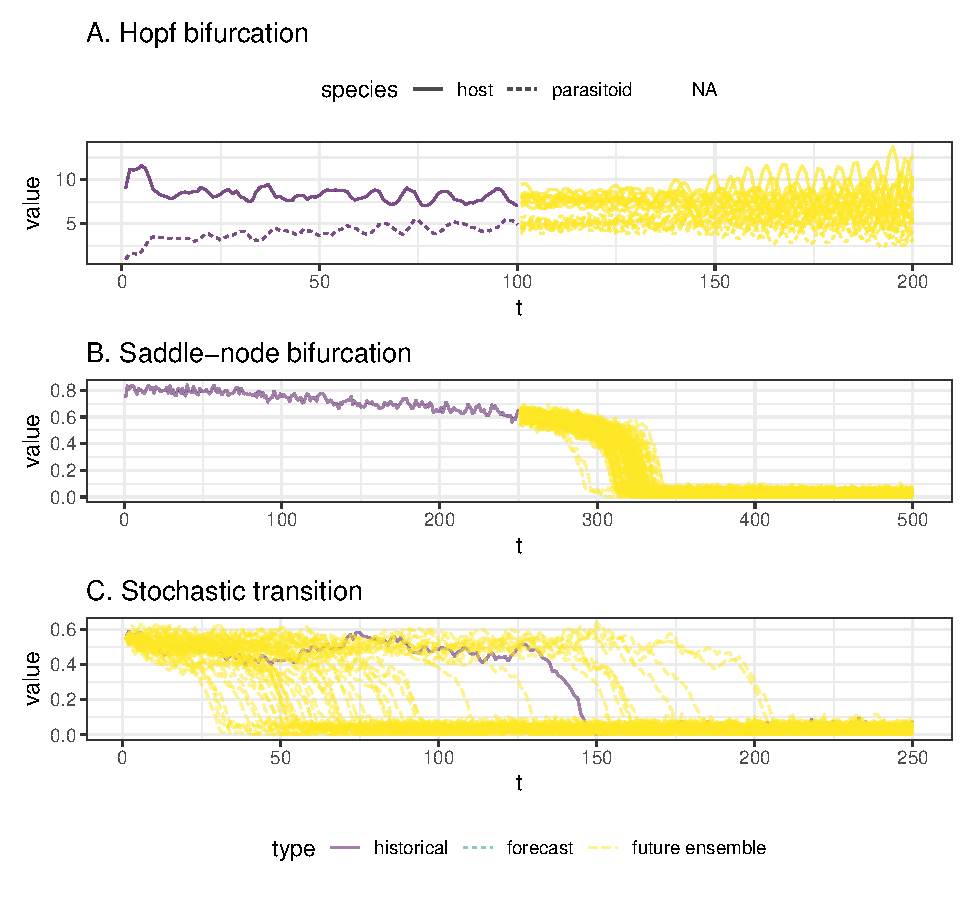
\includegraphics{manuscript_files/figure-latex/figure1-1.pdf}
\caption{Forecast scenarios. A. The Hopf bifurcation: a stable node
develops into a limit cycle which gradually grows larger in this
predator-prey model. B. The saddle-node bifurcation in a single species.
C. The stochastic transition in a single species. Plots show historical
data used to train the algorithm in purple, and replicate simulations of
the true dynamics (`future ensemble') in yellow. Note how the
characteristic time for the critical transition varies across the
transitions. We will examine forecasts of various models (Fig 2) which
will each produce probablistic forecast distributions (blue, Fig 3-5)
seeking to match the true future ensemble (yellow) as closely as
possible.}
\end{figure}

\hypertarget{scenario-1-hopf-bifurcation}{%
\subsection{Scenario 1: Hopf
Bifurcation}\label{scenario-1-hopf-bifurcation}}

The Nicholson-Bailey model describes a predator-prey dynamic for the
relationship of a host species and an obligate parasitoid, originally
used to model the population dynamics of blowflies (\emph{Lucilia
cuprina}) (A. J. Nicholson and Bailey 1935; A. Nicholson 1954a, 1954b).
We consider the form which includes density dependence in the host
species, and allow for environmental stochasticity,

\begin{align}
H_{t+1} &= H_t \exp \left( r \left(1 - \tfrac{H}{K_t}\right) - c P_t + \eta_{H,t} \right) \\
P_{t+1} &= H_t \exp \left( r \left(1 - \tfrac{H}{K_t}\right) \right)  \left(1 -  \exp \left(- c P_t + \eta_{P,t}\right) \right) \\
K_{t+1} &= K_t + \delta
\label{hopf}
\end{align}

Where \(H_t\) is the population density of the host species at time
\(t\), (in arbitrary units) and \(P_t\) the population density of the
parasitoid. The time step is defined by the generation time of the
parasitoid, which is about two weeks in the case of Nicholson's
blowflies (A. Nicholson 1954a). Following Dakos et al. (2012), we
further allow the carrying capacity of the host, \(K\) to slowly
increase at a linear rate, which drives a supercritical Hopf bifurcation
as \(K\) becomes sufficiently large. In a Hopf bifurcation, a stable
node starts an oscillatory pattern which grows in amplitude as the
bifurcation parameter continues to increase. In this model, the Hopf
bifurcation is dubbed `supercritical' as it creates a stable limit cycle
instead of an unstable one. This example illustrates one of the many
kinds of challenges which nonlinear phenomena pose to forecasting: the
``historical'' data prior to the bifurcation never exhibit the cyclical
dynamics of growing amplitude that will emerge after the bifurcation
occurs. If we had used a purely deterministic model, the dynamics would
be constrained to a single stable point, corresponding to a slowly
changing steady-state population size of host and parasitoid
populations. However, stochasticity in this case acts as a source of
some additional information about the dynamics, as the noise excites
quasi-cycles which are visible in the irregular oscillations that appear
significantly prior to the emergence of true limit cycles which follow
the bifurcation (Boettiger 2018b). Examples use the following
parameters: \(H_0 = 9\), \(P_0 = 1\), \(r = 0.75\), \(c = 0.1\),
\(K_0 = 14\), \(\delta = 0.08\), \(\sigma_H = 0.02\),
\(\sigma_P = 0.02\).

\hypertarget{scenario-2-the-saddle-node-bifurcation}{%
\subsection{Scenario 2: The saddle-node
bifurcation}\label{scenario-2-the-saddle-node-bifurcation}}

A yet more difficult forecasting scenario is created by the saddle-node
bifurcation. May's consumer-resource model is an one-dimensional model
describing the growth of a `resource' population (e.g.~herbivore) which
is grazed by a consumer (Robert M. May and Anderson 1979). As in the
Nicholson-Bailey model, in the absence of that predation, the resource
population density grows under a density-dependent pattern described by
a logistic function. The resource population is also grazed by a
consumer at a rate given by a Holling type III s-curve (typically used
to model handling time). For a certain range of parameter choices, this
model supports alternative stable state dynamics, and has been
identified and employed in explaining alternative stable state dynamics
in a broad range of ecological and socio-ecological systems (Scheffer et
al. 2001b).

\begin{align}
N_{t+1} &= N_t + r N_t \left(1 - \frac{N_t}{K} \right) - \frac{h_t N_t^2}{s^2 + N_t^2} + \eta_t \\
h_{t+1} &= h_t + \alpha \\
\eta_t &\sim \mathcal{N}(0, \sigma)
\end{align}

If the environment slowly alters one of the parameters (say, the
encounter efficiency, \texttt{h\_t}, in our formulation), one of the
stable nodes moves closer and closer to the unstable saddle point,
leading to a bifurcation that destroys the stable state, leaving the
system to suddenly transition to the alternative stable state.
Saddle-node bifurcations (also known as fold bifurcations) also create a
phenomenon known as hysteresis, where it is not sufficient to restore
the environment to the previous parameter values to recover the previous
state. Unlike the supercritical Hopf bifurcation which exhibits a
continuous transition from a stable node to a small limit cycle that
then grows, the saddle-node transition is a discontinuous or so-called
`catastrophic' bifurcation. Due both to this sudden, catastrophic nature
of the transition and the difficulty in reversing the shift after it has
occurred, saddle-node bifurcations have been the subject of intense
study.

Tipping point dynamics have long been identified as an important but
difficult challenge for forecasting (e.g. Scheffer et al. 2001a; Folke
et al. 2004). Much effort in the ecological literature so far has
focused on identifying any `early warning signs' that a catastrophic
bifurcation might occur at all (Scheffer et al. 2009, 2012) rather than
more ambitious attempts to provide quantitative probabilistic forecasts
of the likely distribution of waiting times before such a transition
occurs. Tipping points resulting from saddle-node bifurcations have been
demonstrated in examples ranging from laboratory microcosms (Dai et al.
2012; Dai, Korolev, and Gore 2015) to whole-ecosystem experiments
(Carpenter et al. 2011), and postulated as a model for global change
(Barnosky et al. 2012). Examples use the following parameters:
\(r = 1\), \(K = 1\), \(s = 0.1\), \(h_0 = 0.15\),
\(\alpha = 0.000375\), \(\sigma = 0.02\), \(N_0 = 0.75\).

\hypertarget{scenario-3-the-stochastic-transition}{%
\subsection{Scenario 3: The stochastic
transition}\label{scenario-3-the-stochastic-transition}}

Perhaps the most difficult of all events to predict are those in which
large transitions are predominately driven by a random component. An
example of such a transition event is possible to observe in May's
consumer-resource model, in which a stochastic term occasionally results
in a transition between alternative stable states. In such cases, no
forecast can precisely predict when a transition will occur, but it is
nonetheless possible to deduce the correct distribution of waiting times
knowing the correct model. In the case of small noise, transitions are
Poisson distributed, such that the distribution of waiting times is
roughly exponential (e.g. Kampen 1992), though post-hoc the trajectories
of such transitions can be mistaken for saddle-node transitions
(Boettiger and Hastings 2012). To consider such cases, we will again use
May's alternative stable state model, though this time leaving all
parameters fixed.

In this context, predicting the probability of a transition in the
future based solely on observations prior to a transition occurring is
essentially impossible without additional information constraining the
model estimate, as such data is equally consistent with infinitely many
models or parameter choices which share the same local linearization
about the stable point. Unlike the saddle-node bifurcation, there is no
slowly warping potential basin which can be detected to inform
estimates. Thus, in this scenario, rather than considering the problem
of predicting the future evolution of a single time series based only on
its historical values, we consider an alternative framing of the task:
we imagine our forecaster has access to historical data from one or more
comparable systems which includes a previous stochastic transition
event. Based on this data, our forecaster seeks to identify the
distribution of expected transition times for analogous systems starting
from the same initial condition. This parallels actual practice in which
researchers would draw on previous examples of stochastic transitions in
a system - lake-ecosystem shifts, disease emergence, changing fire
regimes, (Scheffer et al. 2001a; Folke et al. 2004). (Note that such
stochastic transitions between alternative stable states can also create
oscillatory-like dynamics when stochasticity is sufficiently high enough
to drive repeated transitions from one attractor to the other and back
again. In such cases, it might be reasonable to estimate a strictly
forward-looking forecast of a single system, predicting the distribution
of these transitions.) Model definition is the same as May's model for
the saddle node with fixed parameter \(h\), values: \(r = 1\),
\(K = 1\), \(s = 0.1\), \(h_0 = h = 0.26\), \(\alpha = 0\),
\(\sigma = 0.02\), \(N_0 = 0.55\).

\textbf{Selecting timescales} In each scenario, t = 0 is the start time
of the training data, while the length of training data and forecast
horizon (with ensembles sampled from the true distribution) is
illustrated in Fig 1. For the Hopf bifurcation, forecast begins at t=100
and extends to t =200, for the saddle node, forecast begins at t=250 and
extends to t = 500, for the stochastic transition, both training data
and forecasting tasks begin at 0 and extend to t = 250. While much
attention is often paid to the number of data points in training or
testing data, it is essential to realize that these are only meaningful
relative to the specific process in question. Thus, in each case we have
selected these time intervals to focus on the dynamical process in
question, which unfolds at a different rate and tempo in each scenario.
For instance, if the stochastic scenario was restricted to a much
shorter timescale used in the Hopf case, few replicate simulations would
experience a transition at all. If it were made much longer, most of the
timeseries would be spent post-transition. Likewise, if the forecast for
the Hopf scenario was extended much further into the future under the
current parameterization, the system experiences a homoclinic
bifurcation at which the population collapses to 0. Using different
length timescales allows us to consider the three different forecasting
tasks illustrated in Fig 1 that focus around predicting the critical
behavior, rather than predicting long periods of relative stasis. These
three critical transitions are fundamentally different processes, there
is no perfect apples-to-apples parameterization for each that allows the
transition to unfold in a way that gives precisely the same time
windows.

\hypertarget{method-group-1-markov-chain-monte-carlo}{%
\subsection{Method group 1: Markov Chain Monte
Carlo}\label{method-group-1-markov-chain-monte-carlo}}

As a reference case, we consider forecasts produced by MCMC estimates of
model parameters, \emph{given the true model}. This represents an
idealized case where the nature of the underlying process is known
precisely. Uncertainty comes from parameter estimates and intrinsic
stochasticity specified in the model, but does not reflect any
uncertainty in our knowledge of the model structure. Alternative model
structures, even when capable of producing the same nonlinear phenomena
(i.e.~the same bifurcations) will give very different forecasts. Even
alternative prior distributions of the parameters will generally yield
alternate forecasts, as likelihood ridges are common to nonlinear
models. Thus, this case represents a theoretical upper bound for the
performance of forecasts by techniques which do not make such strong
assumptions about the underlying processes.

\hypertarget{method-group-2-statistical-models-arima}{%
\subsection{Method group 2: Statistical models
(ARIMA)}\label{method-group-2-statistical-models-arima}}

We present forecasts produced by ARIMA models as the model-free analogs
to the forecasts made using parameter estimation with MCMC. Since ARIMA
models make the assumption that the future will resemble the past via
ARIMA's auto-regressive and moving average components (Hyndman and
Athanasopoulos 2018), these models are not well-suited for problems with
complex bifurcation dynamics. Thus, ARIMA-based forecasts should be
treated as a lower bound for the performance of non-mechanistic models.
In contrast to inference with MCMC, uncertainty with ARIMA models is
estimated directly from the learned parameters (Hyndman and
Athanasopoulos 2018). Since ARIMA is a commonly encountered method, we
will refer readers to Hyndman and Athanasopoulos (2018) for further
discussion.

\hypertarget{method-group-3-machine-learning-models}{%
\subsection{Method group 3: Machine Learning
models}\label{method-group-3-machine-learning-models}}

Over the past decade, deep learning has become very popular for a broad
range of challenging time series prediction problems (Makridakis,
Spiliotis, and Assimakopoulos 2018). Deep learning models are often used
to make point forecasts, but for their application to ecological time
series, it will often be necessary to use multi-step, probabilistic
forecasts. For all the deep learning models in this study, we use the
same general process. Each machine learning model is trained on one time
series drawn from the three scenarios described previously. For the Hopf
and saddle node cases, these time series consist of the period leading
up to the bifurcation. A critical transition is, however, included in
the training set for the stochastic transition case. Each model is
trained to learn the parameters of a Laplace distribution for every time
step in the forecast horizon. To produce a forecast, we input a time
series into a model, then we draw samples from the distributions that
were learned during training.

A major nuisance with deep learning methods is their instability to
hyperparameters and initialization seeds (Madhyastha and Jain 2019). We
found that for the same set of hyperparameters, we could produce starkly
different forecasts if we trained two models with different
initialization seeds. One explanation for this instability is that
machine learning models often get stuck on the local optima of loss
surfaces (Madhyastha and Jain 2019). Another likely cause is that
machine learning models commonly overfit the training data (Mehta et al.
2019). Across deep learning, overfitting is a fundamental issue, arising
from neural networks being highly overparameterized (Dar, Muthukumar,
and Baraniuk 2021). With so many parameters, deep learning models tend
to have high variance and thus overfit the training data, a consequence
of the bias-variance trade-off common across statistics and machine
learning (Mehta et al. 2019). One frequently used method to reduce
overfitting is K-fold cross validation (Raschka 2020), but this approach
cannot be effectively employed when there is one or few time series in
the training set. To remedy the instability problem, we use an
ensemble-based method, wherein each ML forecast is the union of
forecasts from 5 individual models that were trained with different
initialization seeds. We found this simple ensemble technique to be an
effective way to improve generalizability in the limited data regime.

Recently, it has become established that using memory or attention-based
neural networks, and an encoder-decoder architecture is crucial for
improving forecasting performance on time series data (Kao et al. 2020;
Lyu et al. 2020; Du et al. 2020). Herein we will provide some background
on what these machine learning methods are and their benefits.

\hypertarget{recurrent-neural-networks}{%
\subsubsection{Recurrent Neural
Networks}\label{recurrent-neural-networks}}

Recurrent neural networks are the predominant memory-based deep learning
method. Recurrent neural networks differ from feed-forward neural
networks in that a recurrent neural network provides feedback to itself
between time steps (Sherstinsky 2020). By providing self-feedback,
recurrent neural networks are able to retain information from previous
time steps and thus learn temporal dependencies. However, a standard
recurrent neural network is unwieldy to train because of the vanishing
and exploding gradient problem (Pascanu, Mikolov, and Bengio 2013), so
there have been specialized neural network architectures designed to
avoid these gradient problems. Long Short-term Memory and Gated
Recurrent Units Networks are considered to be the state of the art
recurrent neural networks that address exploding and vanishing gradients
(Chung et al. 2014). These methods avoid gradient problems by regulating
the self-feedback via gates which perform operations on the feedback
signal -- see Chung et al. (2014) for more details. While GRU's and
LSTM's commonly outperform standard RNN's, it is difficult to anticipate
whether GRU's or LSTM's will be best suited for any time series problem
(Chung et al. 2014), so we investigate both methods.

\hypertarget{transformers}{%
\subsubsection{Transformers}\label{transformers}}

The Transformer is a state of the art ML architecture that is able to
model long and short term dependencies on sequence to sequence tasks
(Vaswani et al. 2017). Transformers use a mechanism called
self-attention which interrelates different positions of the input
sequence in order to find an informative representation of the input
sequence (Vaswani et al. 2017). For example, if given a sentence, a
transformer could learn the contextual relationship between a subject
and a direct object, but a recurrent neural network would process all
the words as one phrase. Because of self-attention, Transformers do not
need to process data sequentially and thus can be parallelized, offering
significant computational advantages (Vaswani et al. 2017). The
Transformer is likely to be a foundational method for future AI research
(Bommasani et al. 2021), so we considered it critical to investigate
Transformers in this study.

\hypertarget{encoder-decoder}{%
\subsubsection{Encoder-Decoder}\label{encoder-decoder}}

Encoder-decoder architectures have been shown empirically to excel on
sequence to sequence tasks (Aitken et al. 2021). Encoder-decoders work
by processing the input sequence into a fixed-length vector then
decoding the fixed-length vector to the predicted output sequence. It is
thought that by encoding the input sequence to a vector,
encoder-decoders find informative representations of the input sequence
that make the prediction task much easier (Sutskever, Vinyals, and Le
2014). Note that it is possible to use any type of neural network as the
encoder and the decoder, but it is most common to use recurrent neural
networks or networks with attention mechanisms (Aitken et al. 2021). Of
the models that we present, Block RNNs and Transformers have
encoder-decoder-based architectures.

\hypertarget{forecast-skill-strictly-proper-scores}{%
\subsection{Forecast skill: strictly proper
scores}\label{forecast-skill-strictly-proper-scores}}

To compare forecasts, we focus exclusively on metrics of forecast skill
which satisfy the property from Gneiting and Raftery (2007) of a
strictly proper score. This ensures the very desirable behavior that no
probabilistic forecast \(Q(x,t)\) can have a score as high as the score
of the true process \(P(x,t)\) on average. In other words, while it is
possible for any of the models considered to \emph{overfit} the data
against which they are trained, i.e.~have a higher likelihood than the
true process, it is not possible for these models to overfit the data
against which they are scored. It is worth noting that this property
applies specifically to probabilistic forecasts and not point forecasts.
Not all common metrics often used to compare forecasts are strictly
proper -- such as the average root-mean-square error or the average
absolute error. Concerns about over-fitting arise in most types of model
estimation and are a particularly acute concern to machine learning
methods due to the bias-variance trade-off (Mehta et al. 2019). This
makes the use of strictly proper scoring especially relevant in
assessing machine learning predictions.

Not even all strictly proper scores will agree on the same relative
ranking between forecasts. We will focus on two of the most common such
skill metrics, CRPS score and log probability score (negative log
likelihood) (e.g.~see Gneiting and Raftery 2007; Gneiting and Katzfuss
2014). Of the two, the logs probability score puts a much a greater
penalty on unexpected observations than CRPS, and may be more suitable
when the occurrence of unexpected events incurs a particularly high
cost. Note that while the minus log-likelihood can be negative for
sufficiently high probability densities, we use a fixed scalar shift of
logs score to ensure the log skill score is strictly positive, which
facilitates visualization without impacting relative rankings.

\hypertarget{results}{%
\section{Results}\label{results}}

We examine forecast skill for each of the six forecasting methods (MCMC,
ARIMA, block-RNN, GRU, LSTM, and Transformer) in each of our three
scenarios (Hopf bifurcation, saddle-node bifurcation, and stochastic
transition). In addition to these cases, we also consider an ``ensemble
model'', generated by drawing from the distribution of all models except
the MCMC model. Such ensemble techniques can better reflect uncertainty
than relying on any single method (Gneiting and Raftery 2005). For
simplicity, we consider the unweighted case, where each model is
represented equally in the ensemble. Using model-based simulations
allows us to examine performance against multiple (n=100) replicates of
the ``true'' process, which further helps identify differences that may
occur solely due to chance. By taking the true model structure as given,
MCMC methods can be used to determine a theoretical limit of forecasting
skill. Note that in both bifurcation scenarios, future dynamics will
visit states never previously observed in the historical data that was
used to train each of the methods (e.g.~very small population sizes).
This no-analog aspect of forecasting bifurcation dynamics means that
even with many sample points in the training data \emph{and} perfect
knowledge of the true model structure, posterior distributions of
parameter values are still influenced by the choice of priors.

\begin{figure}
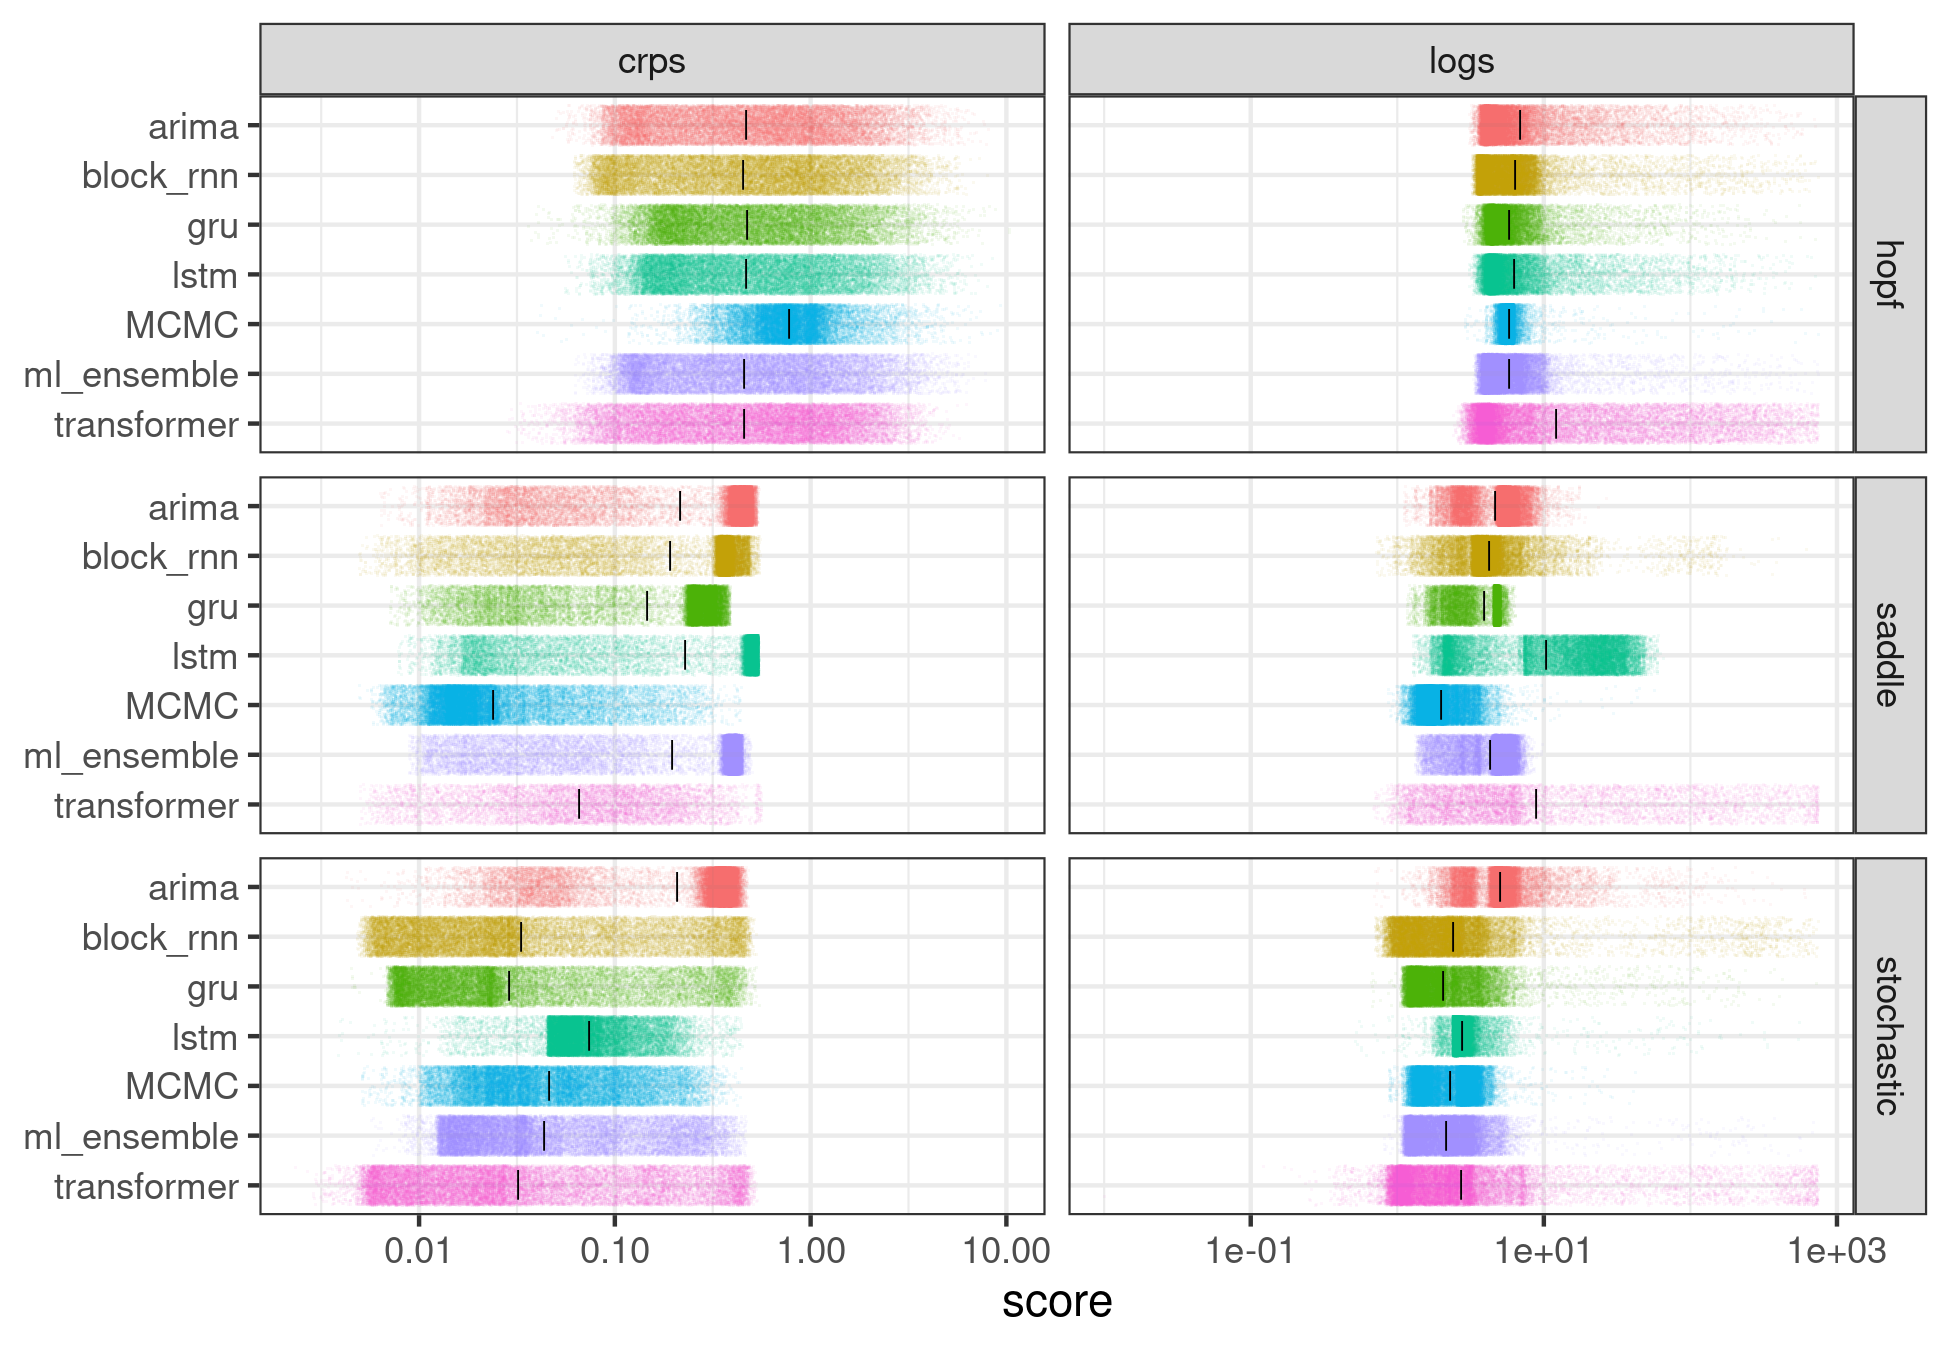
\includegraphics[width=400px,height=300px]{manuscript_files/figure-latex/figure2-1} \caption{Overall distribution of skill scores across models, including an ensemble of methods. Smaller scores are better (indicating smaller errors). Black bars indicate means, dots indicate all individual predictions over time and replicate 'true'simulations of the given scenario.}\label{fig:figure2}
\end{figure}

Overall forecasting skill scores for each model across all three
scenarios are summarized in Fig 2. Average scores (black lines) hide
wide variation in forecast skill. Generally, ML performance tends to be
bracketed between MCMC (essentially the theoretical optimum), and the
statistical ARIMA model, though sometimes performing worse than ARIMA or
better than MCMC. Under scenarios with alternative stable states (saddle
and stochastic), the distribution of scores is often bimodal for ML
models, though not MCMC. The ML ensemble model often performs as well as
the best ML model on average. Note that a wide prediction of uncertainty
does not mean a wide range in the score skill -- for instance the
ensemble model which has the widest array of outcomes often has a
relatively tight distribution of score, especially in logs skill. This
reflects the relative contributions of accuracy and uncertainty as
components in the forecasts. Most ML scores are comparable to MCMC skill
except for the scenario of the saddle-node bifurcation, where all other
models are much worse. Th get a deeper understanding of these general
patterns, we now turn to examine each of the forecast distributions
themselves in comparison to the future ensemble produced by the true
generative process model, Fig 3-5.

\begin{figure}
\centering
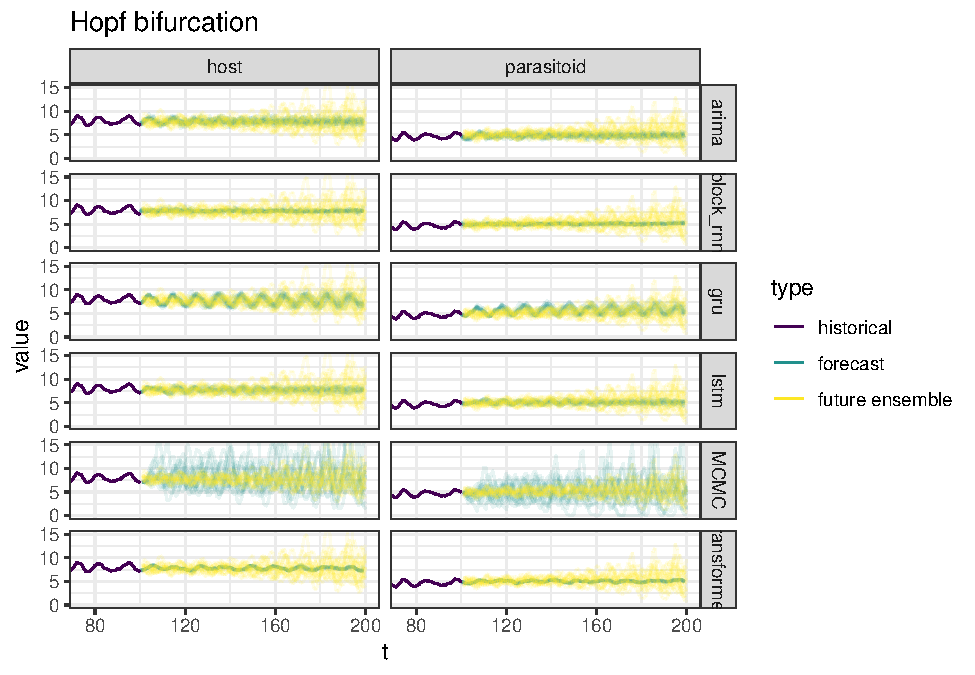
\includegraphics{manuscript_files/figure-latex/figure3-1.pdf}
\caption{Forecasts of the Hopf bifurcation under each model, compared to
15 realizations of the true model. The bifurcation occurs soon after
forecasting period begins,leading to progressively larger and larger
oscillations. Prior to the bifurcation, pseudo-cycles are visible in the
training data due to stochastic excitations. Following the bifurcation,
stochasticity blurs the oscillatory pattern across replicate
simulations. Only last 25 time points of training data are shown.}
\end{figure}

Forecasts of the Hopf bifurcation (Fig 3) are roughly comparable across
the phenomenological models (ARIMA and machine learning models). All
models are trained using 100 time points drawn from the period of time
prior to the onset of the Hopf bifurcation, which leads to a stable
limit cycle that gradually grows in magnitude. Most models predict a
roughly constant mean with a spread roughly equal to that created by the
stochastic oscillations around the stable node as seen in the training
data prior to the bifurcation. Notably, the GRU method picks up the
oscillatory nature of the dynamics, despite the fact that no true
oscillations were yet present in the training data. However, like the
other ML models, it fails to predict the growing amplitude of those
oscillations. Having access to the true model structure, the MCMC model
alone predicts the transition into a pattern of oscillations which grows
over time, though it tends to overestimate the amplitude of those
oscillations initially. Despite this, overall all methods score
comparably in CRPS score (Fig 2), with most ML methods actually
out-performing the MCMC score on average (Fig 5), albeit with much
greater variation in individual scores. A clearer picture can be seen by
looking at these skill scores over time (Fig 6-7), which show that MCMC
is initially performing worse (over-predicting variance) but as
oscillations grow further, it starts outperforming the more stationary
forecasts of the ML models.

\begin{figure}
\centering
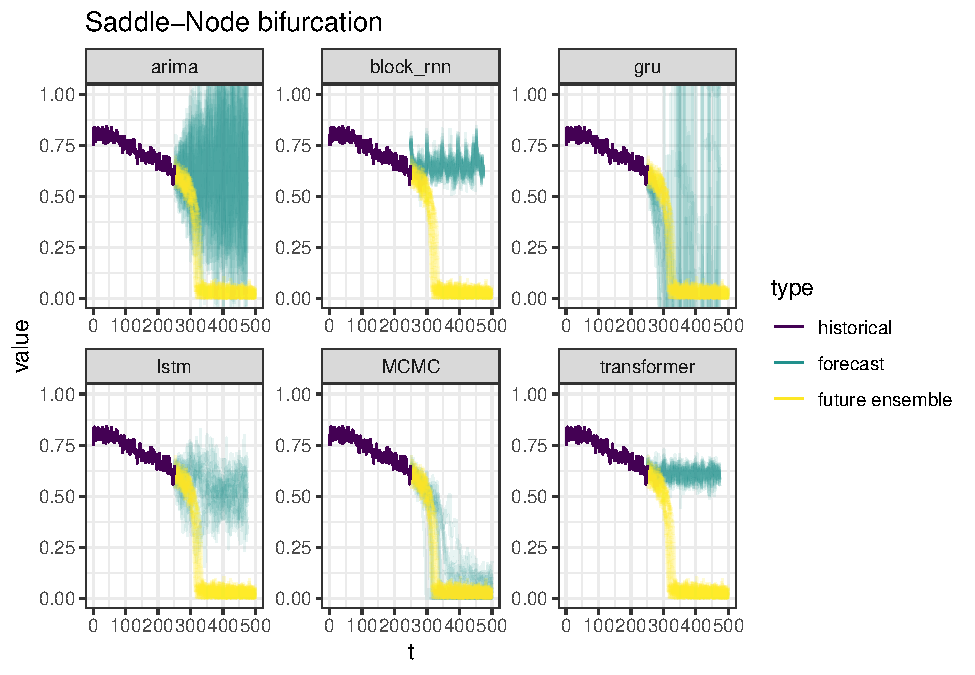
\includegraphics{manuscript_files/figure-latex/figure4-1.pdf}
\caption{Forecasts of the saddle-node bifurcation under each model,
compared to 15 realizations of the true model. Training data proceeds
the bifurcation, making accurate prediction without knowledge of the
underlying model very difficult.}
\end{figure}

The saddle node bifurcation proves even more difficult for most methods
(Fig 4). Only the MCMC model anticipates the sharp transition to an
alternative state, though this behavior is more baked into the method
from the start which takes the true model structure as given. Even
accurate estimation of the MCMC requires slightly informative priors,
though still broad enough to reflect a wide range of possible outcomes.
Two ML methods -- Block RNNs and Transformers -- resemble a naive
prediction extrapolating the last observed state, failing even to
reflect the slow downward trend of the training data. LSTM indicates
greater uncertainty, while GRU shows very large variability which spans
the alternative stable state range. With additional tuning, better
performance may be possible for these ML models. The selected ARIMA
model reflects wide uncertainty that is nevertheless not broad enough to
span the alternative stable state. Consequentially, the MCMC estimate
easily outperforms the ML models (Fig 2).

\begin{figure}
\centering
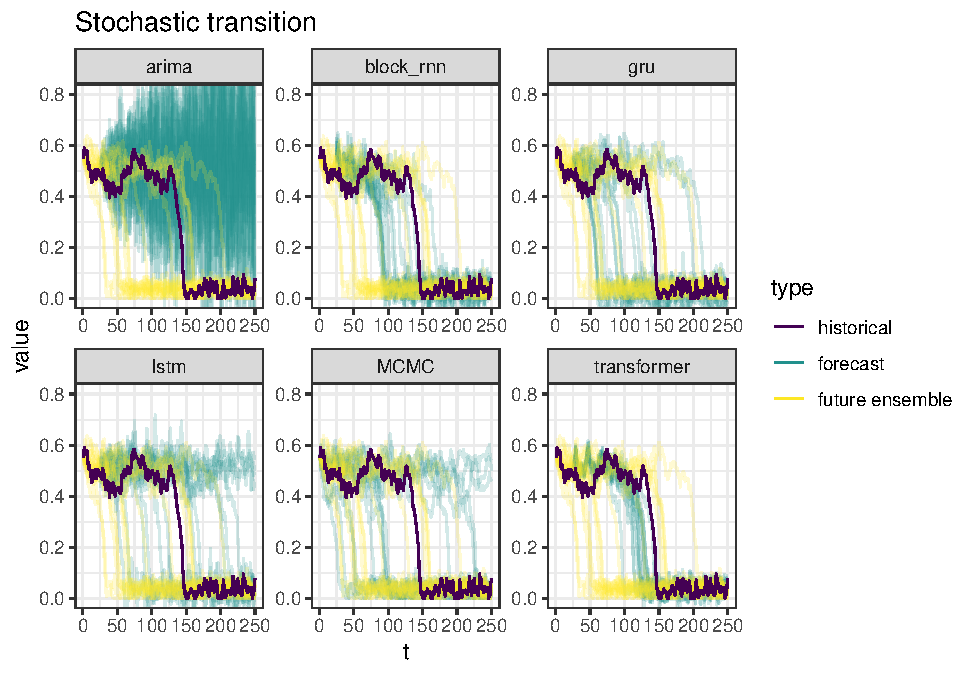
\includegraphics{manuscript_files/figure-latex/figure5-1.pdf}
\caption{Forecasts of the stochastic transition under each model,
compared to 15 realizations of the true model. In contrast to the other
challenges, this case considers the prediction of replicate systems
starting from the same initial condition, rather than forecasting the
future evolution of the model after the stochastic transition has
already occurred.}
\end{figure}

Machine learning methods do markedly better on the stochastic transition
scenario than in the two bifurcation scenarios (Fig 5). This occurs
because the training data includes the transition phenomenon of
interest. All ML models accurately capture the dynamics of a sharp
transition between alternative stable states -- a dynamic the
statistical ARIMA model entirely fails to reflect. Stochastic transition
events should be approximately exponentially distributed, as seen in the
wide range of waiting times for transitions to occur in replicates of
the true `observed' process (Fig 5). Transformer and Block RNN
distribution times are much more concentrated, while again GRU and
especially the LSTM do a better job reflecting the uncertainty in range
of transition times.

Examining patterns in the scores over time (Fig 6-7) provides a more
nuanced understanding of the forecast dynamics than aggregate scores
alone (Fig 2). In the Hopf bifurcation, CRPS scores get worse over time
across all methods, including the MCMC forecasts. In the saddle node
bifurcation and stochastic transition, the same pattern holds somewhat
more dramatically for non-MCMC forecast, while MCMC scores are worst in
mid-range. Comparing CRPS scores to logs score also emphasizes the
relative role of uncertainty: for instance, the MCMC scores for the Hopf
bifurcation get steadily worse under CRPS but not under logs score. A
relatively sharp transition can be seen under both MCMC scores on the
Hopf bifurcation once the magnitude of the oscillations exceeds the
variance created by mere stochasticity: the MCMC model no longer
over-estimates the spread of the data, while the ML models now
underestimate that variation. CRPS scores for stochastic transitions
exhibit a distinct two-branch pattern, with scores for a given replicate
being either very high (poor skill) or very low, reflecting whether the
individual `true' replicate matches the mean state predicted by the
forecast or the other state. Logs skill score may be a better measure in
this context, where correctly capturing the uncertainty in the forecast
means that this bi-modal structure in scores can be avoided entirely,
e.g.~by the MCMC predictions. The forecast-skill-over time plots
illustrate different reasons for the bi-modal distribution in skill seen
for the saddle-node and stochastic transition scenarios in Fig 2
respectively: in the case of the saddle node, the two modes are
distinguished by time-horizon: short term forecasts are relatively
accurate, longer term forecasts (i.e.~after the catastrophic transition)
are poor. In the case of the stochastic transition model, the two modes
are not structured by horizon but by replicate, with some replicates
having transitioned and others still in the original state.

\begin{figure}
\centering
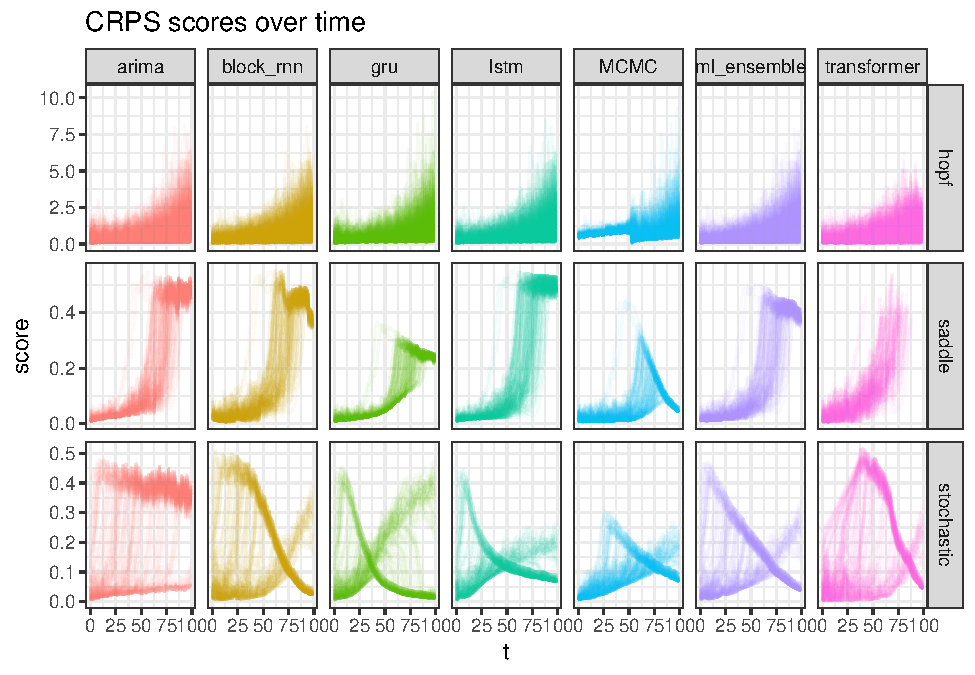
\includegraphics{manuscript_files/figure-latex/figure6-1.pdf}
\caption{CRPS scores over time for each scenario. Each line represents
the scores against a replicate of time series observations from `true
model'. Patterns show forecast skill generally get worse over time --
graduallyin the case of Hopf bifurcation or suddenly in response to the
saddle-node bifurcation. The MCMC shows a sharp improvement in forecast
skill over time as it passes the transition window. In the stochastic
transition context, this creates two branches, where high values
indicate periods oftime when the forecast predicts the wrong state and
lower branch indicates the correct state.}
\end{figure}

\begin{figure}
\centering
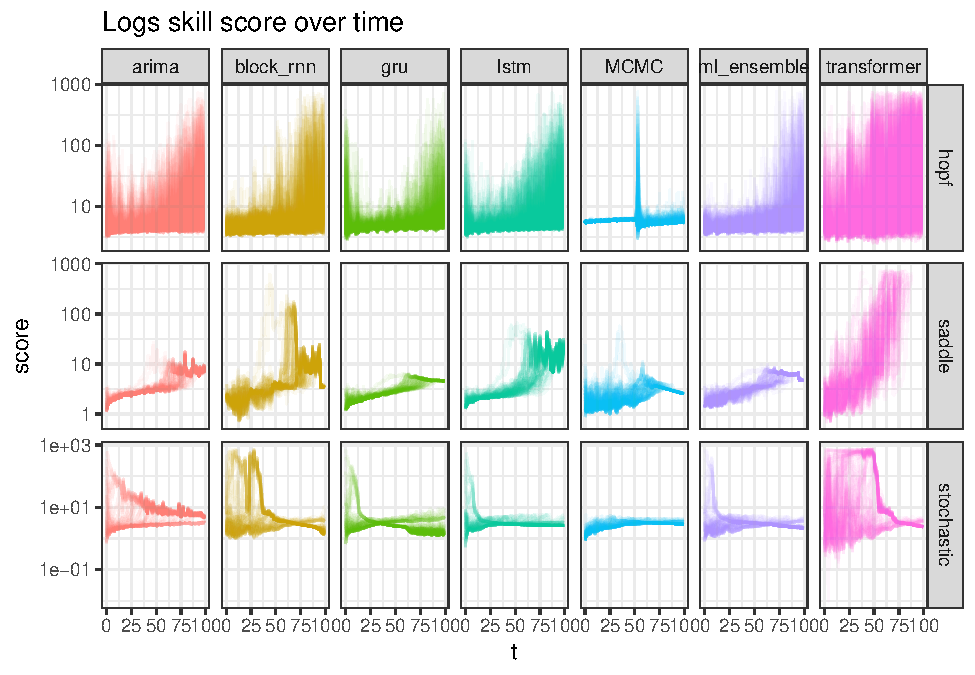
\includegraphics{manuscript_files/figure-latex/figure7-1.pdf}
\caption{Logs skill score over time. Forecasts which underestimate
uncertainty do substantially worse in logs score than in CRPS score.
Comparing this panel to those in Fig 6 highlights scenarios that most
often underestimate uncertainty. Generally, MCMC performs better
relative to other models under this metric than it does under
CRPS,reflecting the bias-variance tradeoff of machine learning.}
\end{figure}

\hypertarget{discussion}{%
\section{Discussion}\label{discussion}}

Ecological systems have long been acknowledged as complex, due not only
to the immense span of dimension and scale such processes involve, but
also the frequency of emergent and non-linear phenomena such as
stochastic resonance, including bifurcations, tipping points, and
hysteresis examined here. Calls for increased forecasting efforts from
ecologists frequently reference the role of changing climate and other
anthropogenic change, which raise the challenge of prediction in
no-analog environments, anticipating ecosystem responses to conditions
that have not been previously observed (Clark et al. 2001; Dietze et al.
2018). This motivates the question, ``What methods will be most reliable
in the face of unobserved conditions?''

In this paper, we carry out an initial exploration on how deep learning
methods can perform on predicting critical transition events. We compare
the ability of several cutting edge machine learning approaches against
statistical and process-based models, and show that deep learning
methods are generally able to strike a middle ground between what we
consider as acceptable and ideal case forecasting methods, ARIMA and
MCMC-based parameter estimation respectively. Although most ML-based
forecasting applications focus on point predictions, we have emphasized
examples that can provide estimates of uncertainty. When the ML models
are able to observe transition phenomena, as in the stochastic case,
they performed comparably to MCMC-based forecasting with respect to CRPS
and log probability score but under-performed MCMC when there were no
transition events in the training sets as in the Hopf and saddle-node
examples. An ensemble forecast combining the predictions of all four ML
methods generally scores as well or better than any one of the ML
methods alone. Yet, examining summary statistics, CRPS and log
probability scores obscures finer detailed components of the forecasts.
For instance, forecast skill varies with the length of the forecast
horizon in a non-monotonic fashion. This is the result of multiple
factors: for some dynamics, such as those involving tipping points, the
long term behavior can be easier to predict than transient transitions.
Both predicted uncertainty and forecast skill can be better on longer
horizons than on shorter ones, as in the MCMC predictions of tipping
point dynamics. It is also important to remember that probabilistic
forecast skill scores do not only measure how close observations are to
expectation, but also reflect the predicted uncertainty: therefore,
over-confidence about predictive accuracy can result in worse scores
than scores from forecasts that are less accurate on average but
correctly reflect a greater degree of uncertainty. The ability to better
reflect uncertainty rather than better average predictions explains much
of the performance of the ensemble model.

The success of these ML models on the stochastic transition case is
particularly notable. All methods are given only a single previous
replicate of a stochastic transition (Fig 5, red line) on which to base
their estimates. This is typical of ecological scenarios where data is
so often limited. While even one observation of a transition is more
than the methods have in our other forecasts, this still presents a
significant challenge to model estimation. Unlike the MCMC case, the ML
models have no prior expectation of a model structure that contains
sharp transitions -- we might have expected these models to perform
little differently than the ARIMA model. Given this single replicate,
all four ML models successfully capture the phenomenological pattern of
a sharp shift between two stable states -- this is behavior that the
structurally simpler family of ARIMA models cannot express. This
provides a clear illustration of the much broader array of
phenomenological behaviors that can be accurately modeled with ML models
compared to classical statistical models. In this way, the ML models can
be seen as imposing even fewer assumptions on the phenomenological
behavior of the system than the ARIMA model. In contrast, the MCMC
performance benefits from very strong process-based assumptions, which
happen to match the `true' model in this case and thus provide a
comparison of the theoretical optimal performance.

The MCMC case illustrates some of the hard limits to ecological
forecasting of critical transitions. Our MCMC forecast assumes the
\emph{true} model structure, the data-generating process, is known, and
the forecaster need only infer the posterior distribution of model
parameters. This is a much stronger assumption than that made by the ML
models, though this assumption can potentially be justified on the basis
of a mechanistic understanding of the processes involved. It is
important not to confound the MCMC example here with the use of MCMC in
process based models of real systems. In the real world, this is never
the case: all models are at best approximations of the underlying
processes (Oreskes, Shrader-Frechette, and Belitz 1994). Despite this
advantage, even the MCMC forecasts differ from the distribution of the
true process. Because the available data come from only a small region
of the dynamical state space, they are consistent with many possible
parameterizations of the same model structure -- which creates
likelihood ridges and non-identifiability of specific parameter values.
Using more simplified versions of the dynamical processes in question,
such as the canonical form of a bifurcation, can mitigate this issue in
some cases. Even when such non-identifiability issues cannot be avoided
entirely, they can usually be diagnosed by examining the degree of
mixing in MCMC sampling and comparing posterior to prior distributions.

When examining the performance of the ML models, it is clear that there
is no single method that excels in all scenarios. Neither is there one
class of ML methods that outperforms the others -- a fact we found
surprising given the reported dominance of encoder-decoders in the field
of sequence-to-sequence deep learning (Aitken et al. 2021). These
observations underscore the point that ML is a very empirically-driven
field in which there are few guarantees on performance. Furthermore, due
to the black-box-ness of deep learning and other reasons like
instability to initialization seed, it is often impossible to provide an
explanation for why certain methods over-perform or fail to meet
expectations.

Overall, ML models and the more traditional ARIMA model fail to predict
the qualitative shift in dynamic behavior that occurs in the critical
transition scenarios (Hopf and saddle node). This is not surprising, as
the training data provide no prior example of such behavior
(e.g.~growing oscillations or a sudden shift). Nevertheless, this should
be an important reminder of a central difficulty in ecological
forecasting. Note that in such scenarios, near-term forecasts (Dietze et
al. 2018) may be very accurate right up to the transition event before
becoming widely wrong. Nor can the possibility of such non-linear
behavior be easily dismissed in ecological models -- the examples
considered here have been bedrock of ecological modeling and management
practices for over half a century (Folke et al. 2004), and if anything
are only too simple, representing a small slice of possible dynamical
behavior of more complicated models.

It may be natural to ask whether this performance would be remedied if
the ML models were trained on data which includes prior examples of
supercritical Hopf or saddle node bifurcations. This question is not as
easy to answer as it may seem, because of the difficulty in defining the
corresponding forecasting scenario. The scenarios we have considered are
true, pure forecasts: the training data comes from a single realization
of a specific generative process, and the task is to predict the future
states of that system before they occur. Would it be possible to train a
predictive algorithm on `analogous' examples of critical transitions?
For instance, could data from other lakes, which may have experienced a
critical transition such as an eutrophication event in the past, be used
to train machine learning models to predict such events in some focal
lake in the future (Scheffer et al. 2001a)? Perhaps, but it depends on
what we mean by an `analogous' system. Even if the underlying mechanism
was accurately captured by the same model, say, the saddle-node model of
Robert M. May (1977) we consider here, it is likely that most of the
individual model parameters would be quite different, even after
accounting for re-scaling or non-dimensionalization of the model
(Hastings 1996). Rarely do ecologists have access to completely
controlled replicates for fitting or training models. The ability for ML
models to successfully generalize from training in such cases remains an
open problem and a promising subject of further investigation.

There are a number of questions that we have left unanswered that we
hope will be addressed in future work. In this paper, we have explored a
small number of machine learning and statistical models that can be used
for forecasting, so comprehensive conclusions can not be drawn on
whether statistical or machine learning-based approaches are better
suited for critical transition forecasting problems. Neither can we
claim that the ML methods employed will translate well to all sudden
transition event forecasting problems in reality, since working with
real data will introduce additional difficulties like how to deal with
missing data, sparse data and observation errors.

Furthermore, our analysis has focused on the task of making a single
forecast prior to the occurrence of a critical transition. Forecasting
is ideally a more iterative process of data assimilation, where
forecasts are updated with respect to additional observations, rather
than projecting 100s of time steps into the future (Dietze et al. 2018).
Updating a forecast after a critical transition has already occurred may
be of little use in the context of hysteresis, such as under the saddle
node or stochastic transition -- recognizing the alternative stable
state only after the system is stuck in that basin will often be
considered `too late'. Assimilation may be more applicable to the Hopf
bifurcation, where additional observations of slowly growing
oscillations may lead to more accurate forecasts. Such models may even
accurately predict the homoclinic bifurcation that occurs when the limit
cycle grows too large, eventually hitting a saddle point of zero
population size for the host species. We leave these cases to future
exploration rather than attempting to explore all such variations in a
single narrative. We have focused on these illustrative examples
accompanied by an extensive appendix of reproducible code implemented
using well documented and intuitive frameworks. We encourage the reader
to use these appendices as an entry point into further exploration.

Ecological forecasting is invariably difficult, even in the idealized
cases of ample measurement data and clearly identified structural
models. This paper is not intended to give a complete answer to whether
deep learning is the best suited method for tipping point forecasting
problems as this will take numerous studies to resolve; instead, this
paper aims to be an early exploration on whether deep learning methods
should be considered as viable tools for this extremely challenging
class of prediction problems. Given the difficulty of forecasting
never-before-observed behavior, as illustrated by the Hopf and
saddle-node bifurcation scenarios, there is good reason for research to
focus more on the kind of qualitative predictions long emphasized in the
literature on early warning signals and resilience
(\textbf{scheffer2015?}). Recently, ML techniques developed for
classification rather than the ML methods used in regression and
forecasting models considered here have demonstrated a more nuanced
ability to reliably detect different classes of critical transitions in
time-series data (\textbf{bury2021?}; \textbf{lapeyrolerie2021?}).
Rather than seeking to provide managers with quantitative, probabilistic
forecasts reflecting a broad uncertainty in possible outcomes, this
literature has sought to emphasize only a more qualitative form of
prediction, such as establishing whether a system is either
``resilient'' or ``approaching a critical transition.'' Decision
sciences have long emphasized the importance of reconciling the
qualitative predictions of resilience thinking with quantitative
forecasts of future states (\textbf{folke2009?}; \textbf{polasky2011?}).
Such approaches could be valuable in concert with probabilistic
forecasts considered here, providing a possible mechanism to identify
when the probabilistic forecast is least reliable.

\hypertarget{acknowledgements}{%
\section{Acknowledgements}\label{acknowledgements}}

This material is based upon work supported by the National Science
Foundation under Grant No.~DBI-1942280.

\hypertarget{conflicts-of-interest}{%
\section*{Conflicts of Interest}\label{conflicts-of-interest}}
\addcontentsline{toc}{section}{Conflicts of Interest}

The authors declare there are no conflicts of interest.

\hypertarget{authors-contributions}{%
\section*{Authors' Contributions}\label{authors-contributions}}
\addcontentsline{toc}{section}{Authors' Contributions}

M.L. and C.B. developed the code and wrote the manuscript.

\hypertarget{data-availability}{%
\section*{Data Availability}\label{data-availability}}
\addcontentsline{toc}{section}{Data Availability}

We have created a github repository
\url{https://github.com/boettiger-lab/mee_tipping_point_forecasting.}
that contains the code used to produce the figures herein.

\newpage

\hypertarget{references}{%
\section*{References}\label{references}}
\addcontentsline{toc}{section}{References}

\hypertarget{refs}{}
\begin{CSLReferences}{1}{0}
\leavevmode\vadjust pre{\hypertarget{ref-aitken_understanding_2021}{}}%
Aitken, Kyle, Vinay V. Ramasesh, Yuan Cao, and Niru Maheswaranathan.
2021. {``Understanding {How} {Encoder}-{Decoder} {Architectures}
{Attend}.''} arXiv. \url{http://arxiv.org/abs/2110.15253}.

\leavevmode\vadjust pre{\hypertarget{ref-Barnosky2012}{}}%
Barnosky, Anthony D., Elizabeth A. Hadly, Jordi Bascompte, Eric L.
Berlow, James H. Brown, Mikael Fortelius, Wayne M. Getz, et al. 2012.
{``Approaching a State Shift in {Earth}'s Biosphere.''} \emph{Nature}
486 (7401): 52--58. \url{https://doi.org/10.1038/nature11018}.

\leavevmode\vadjust pre{\hypertarget{ref-Boettiger2018}{}}%
Boettiger, Carl. 2018a. {``From Noise to Knowledge: How Randomness
Generates Novel Phenomena and Reveals Information.''} \emph{Ecology
Letters}. \url{https://doi.org/10.1111/ele.13085}.

\leavevmode\vadjust pre{\hypertarget{ref-boettiger_noise_2018}{}}%
---------. 2018b. {``From Noise to Knowledge: How Randomness Generates
Novel Phenomena and Reveals Information.''} Edited by Tim Coulson.
\emph{Ecology Letters} 21 (8): 1255--67.
\url{https://doi.org/10.1111/ele.13085}.

\leavevmode\vadjust pre{\hypertarget{ref-boettiger_early_2012}{}}%
Boettiger, Carl, and Alan Hastings. 2012. {``Early Warning Signals and
the Prosecutor's Fallacy.''} \emph{Proceedings of the Royal Society B:
Biological Sciences} 279 (1748): 4734--39.
\url{https://doi.org/10.1098/rspb.2012.2085}.

\leavevmode\vadjust pre{\hypertarget{ref-bommasani_opportunities_2021}{}}%
Bommasani, Rishi, Drew A. Hudson, Ehsan Adeli, Russ Altman, Simran
Arora, Sydney von Arx, Michael S. Bernstein, et al. 2021. {``On the
{Opportunities} and {Risks} of {Foundation} {Models}.''}
\emph{arXiv:2108.07258 {[}Cs{]}}, August.
\url{http://arxiv.org/abs/2108.07258}.

\leavevmode\vadjust pre{\hypertarget{ref-bury_2021}{}}%
Bury, Thomas M., R. I. Sujith, Induja Pavithran, Marten Scheffer,
Timothy M. Lenton, Madhur Anand, and Chris T. Bauch. 2021. {``Deep
Learning for Early Warning Signals of Tipping Points.''}
\emph{Proceedings of the National Academy of Sciences} 118 (39):
e2106140118. \url{https://doi.org/10.1073/pnas.2106140118}.

\leavevmode\vadjust pre{\hypertarget{ref-carpenter_early_2011}{}}%
Carpenter, S. R., J. J. Cole, M. L. Pace, R. Batt, W. A. Brock, T.
Cline, J. Coloso, et al. 2011. {``Early {Warnings} of {Regime} {Shifts}:
{A} {Whole}-{Ecosystem} {Experiment}.''} \emph{Science} 332 (6033):
1079--82. \url{https://doi.org/10.1126/science.1203672}.

\leavevmode\vadjust pre{\hypertarget{ref-chung_empirical_2014}{}}%
Chung, Junyoung, Caglar Gulcehre, KyungHyun Cho, and Yoshua Bengio.
2014. {``Empirical {Evaluation} of {Gated} {Recurrent} {Neural}
{Networks} on {Sequence} {Modeling}.''} \emph{arXiv:1412.3555 {[}Cs{]}},
December. \url{http://arxiv.org/abs/1412.3555}.

\leavevmode\vadjust pre{\hypertarget{ref-clark_ecological_2001}{}}%
Clark, James S., Steven R. Carpenter, Mary Barber, Scott Collins, Andy
Dobson, Jonathan A. Foley, David M. Lodge, et al. 2001. {``Ecological
{Forecasts}: {An} {Emerging} {Imperative}.''} \emph{Science} 293 (5530):
657--60. \url{https://doi.org/10.1126/science.293.5530.657}.

\leavevmode\vadjust pre{\hypertarget{ref-Dai2015}{}}%
Dai, Lei, Kirill S. Korolev, and Jeff Gore. 2015. {``Relation Between
Stability and Resilience Determines the Performance of Early Warning
Signals Under Different Environmental Drivers.''} \emph{Proceedings of
the National Academy of Sciences}, 201418415.
\url{https://doi.org/10.1073/pnas.1418415112}.

\leavevmode\vadjust pre{\hypertarget{ref-Dai2012}{}}%
Dai, Lei, Daan Vorselen, Kirill S Korolev, and J. Gore. 2012. {``Generic
{Indicators} for {Loss} of {Resilience} {Before} a {Tipping} {Point}
{Leading} to {Population} {Collapse}.''} \emph{Science (New York, N.Y.)}
336 (6085): 1175--77. \url{https://doi.org/10.1126/science.1219805}.

\leavevmode\vadjust pre{\hypertarget{ref-dakos_methods_2012}{}}%
Dakos, Vasilis, Stephen R. Carpenter, William A. Brock, Aaron M.
Ellison, Vishwesha Guttal, Anthony R. Ives, Sonia Kéfi, et al. 2012.
{``Methods for {Detecting} {Early} {Warnings} of {Critical}
{Transitions} in {Time} {Series} {Illustrated} {Using} {Simulated}
{Ecological} {Data}.''} Edited by Bülent Yener. \emph{PLoS ONE} 7 (7):
e41010. \url{https://doi.org/10.1371/journal.pone.0041010}.

\leavevmode\vadjust pre{\hypertarget{ref-dar_farewell_2021}{}}%
Dar, Yehuda, Vidya Muthukumar, and Richard G. Baraniuk. 2021. {``A
{Farewell} to the {Bias}-{Variance} {Tradeoff}? {An} {Overview} of the
{Theory} of {Overparameterized} {Machine} {Learning}.''} arXiv.
\url{http://arxiv.org/abs/2109.02355}.

\leavevmode\vadjust pre{\hypertarget{ref-dietze_iterative_2018}{}}%
Dietze, Michael C., Andrew Fox, Lindsay M. Beck-Johnson, Julio L.
Betancourt, Mevin B. Hooten, Catherine S. Jarnevich, Timothy H. Keitt,
et al. 2018. {``Iterative Near-Term Ecological Forecasting: {Needs},
Opportunities, and Challenges.''} \emph{Proceedings of the National
Academy of Sciences} 115 (7): 1424--32.
\url{https://doi.org/10.1073/pnas.1710231115}.

\leavevmode\vadjust pre{\hypertarget{ref-du_multivariate_2020}{}}%
Du, Shengdong, Tianrui Li, Yan Yang, and Shi-Jinn Horng. 2020.
{``Multivariate Time Series Forecasting via Attention-Based
Encoder--Decoder Framework.''} \emph{Neurocomputing} 388 (May): 269--79.
\url{https://doi.org/10.1016/j.neucom.2019.12.118}.

\leavevmode\vadjust pre{\hypertarget{ref-Fischer2009}{}}%
Fischer, Joern, Garry D Peterson, Toby A. Gardner, Line J Gordon, Ioan
Fazey, Thomas Elmqvist, Adam Felton, Carl Folke, and Stephen Dovers.
2009. {``Integrating Resilience Thinking and Optimisation for
Conservation.''} \emph{Trends in Ecology \& Evolution} 24 (10): 549--54.
\url{https://doi.org/10.1016/j.tree.2009.03.020}.

\leavevmode\vadjust pre{\hypertarget{ref-Folke2004}{}}%
Folke, Carl, Steve Carpenter, Brian Walker, Marten Scheffer, Thomas
Elmqvist, Lance Gunderson, and C. S. Holling. 2004. {``Regime {Shifts},
{Resilience}, and {Biodiversity} in {Ecosystem} {Management}.''}
\emph{Annual Review of Ecology, Evolution, and Systematics} 35 (1):
557--81. \url{https://doi.org/10.1146/annurev.ecolsys.35.021103.105711}.

\leavevmode\vadjust pre{\hypertarget{ref-Getz2018}{}}%
Getz, Wayne M., Charles R. Marshall, Colin J. Carlson, Luca Giuggioli,
Sadie J. Ryan, Stephanie S. Romañach, Carl Boettiger, et al. 2018.
{``Making Ecological Models Adequate.''} Edited by Tim Coulson.
\emph{Ecology Letters} 21 (2): 153--66.
\url{https://doi.org/10.1111/ele.12893}.

\leavevmode\vadjust pre{\hypertarget{ref-gneiting_probabilistic_2014}{}}%
Gneiting, Tilmann, and Matthias Katzfuss. 2014. {``Probabilistic
{Forecasting}.''} \emph{Annual Review of Statistics and Its Application}
1 (1): 125--51.
\url{https://doi.org/10.1146/annurev-statistics-062713-085831}.

\leavevmode\vadjust pre{\hypertarget{ref-gneiting_strictly_2007}{}}%
Gneiting, Tilmann, and Adrian E Raftery. 2007. {``Strictly {Proper}
{Scoring} {Rules}, {Prediction}, and {Estimation}.''} \emph{Journal of
the American Statistical Association} 102 (477): 359--78.
\url{https://doi.org/10.1198/016214506000001437}.

\leavevmode\vadjust pre{\hypertarget{ref-gneiting_weather_2005}{}}%
Gneiting, Tilmann, and Adrian E. Raftery. 2005. {``Weather {Forecasting}
with {Ensemble} {Methods}.''} \emph{Science} 310 (5746): 248--49.
\url{https://doi.org/10.1126/science.1115255}.

\leavevmode\vadjust pre{\hypertarget{ref-hallett_why_2004}{}}%
Hallett, T. B., T. Coulson, J. G. Pilkington, T. H. Clutton-Brock, J. M.
Pemberton, and B. T. Grenfell. 2004. {``Why Large-Scale Climate Indices
Seem to Predict Ecological Processes Better Than Local Weather.''}
\emph{Nature} 430 (6995): 71--75.
\url{https://doi.org/10.1038/nature02708}.

\leavevmode\vadjust pre{\hypertarget{ref-Hastings1996}{}}%
Hastings, Alan. 1996. \emph{Population {Biology}: {Concepts} and
{Models}}. Springer.

\leavevmode\vadjust pre{\hypertarget{ref-hyndman_forecasting_2018}{}}%
Hyndman, R. J., and G. Athanasopoulos. 2018. \emph{Forecasting:
Principles and Practice}. 2nd ed. Melbourne, Australia: OTexts.
\href{https://OTexts.com/fpp2}{OTexts.com/fpp2}.

\leavevmode\vadjust pre{\hypertarget{ref-kampen_stochastic_1992}{}}%
Kampen, N. G. van. 1992. \emph{Stochastic Processes in Physics and
Chemistry}. Rev. and enl. ed. North-{Holland} Personal Library.
Amsterdam ; New York: North-Holland.

\leavevmode\vadjust pre{\hypertarget{ref-kao_exploring_2020}{}}%
Kao, I-Feng, Yanlai Zhou, Li-Chiu Chang, and Fi-John Chang. 2020.
{``Exploring a {Long} {Short}-{Term} {Memory} Based {Encoder}-{Decoder}
Framework for Multi-Step-Ahead Flood Forecasting.''} \emph{Journal of
Hydrology} 583 (April): 124631.
\url{https://doi.org/10.1016/j.jhydrol.2020.124631}.

\leavevmode\vadjust pre{\hypertarget{ref-Levins1966}{}}%
Levins, Richard. 1966. {``The Strategy of Model Building in Population
Biology.''} \emph{American Scientist} 54 (4): 421--31.

\leavevmode\vadjust pre{\hypertarget{ref-lyu_lstm_2020}{}}%
Lyu, Pingyang, Ning Chen, Shanjun Mao, and Mei Li. 2020. {``{LSTM} Based
Encoder-Decoder for Short-Term Predictions of Gas Concentration Using
Multi-Sensor Fusion.''} \emph{Process Safety and Environmental
Protection} 137 (May): 93--105.
\url{https://doi.org/10.1016/j.psep.2020.02.021}.

\leavevmode\vadjust pre{\hypertarget{ref-madhyastha_model_2019}{}}%
Madhyastha, Pranava, and Rishabh Jain. 2019. {``On {Model} {Stability}
as a {Function} of {Random} {Seed}.''} \emph{arXiv:1909.10447 {[}Cs,
Stat{]}}, September. \url{http://arxiv.org/abs/1909.10447}.

\leavevmode\vadjust pre{\hypertarget{ref-makridakis_statistical_2018}{}}%
Makridakis, Spyros, Evangelos Spiliotis, and Vassilios Assimakopoulos.
2018. {``Statistical and {Machine} {Learning} Forecasting Methods:
{Concerns} and Ways Forward.''} Edited by Alejandro Raul Hernandez
Montoya. \emph{PLOS ONE} 13 (3): e0194889.
\url{https://doi.org/10.1371/journal.pone.0194889}.

\leavevmode\vadjust pre{\hypertarget{ref-May1977}{}}%
May, Robert M. 1977. {``Thresholds and Breakpoints in Ecosystems with a
Multiplicity of Stable States.''} \emph{Nature} 269 (5628): 471--77.
\url{https://doi.org/10.1038/269471a0}.

\leavevmode\vadjust pre{\hypertarget{ref-may_population_1979}{}}%
May, Robert M., and Roy M. Anderson. 1979. {``Population Biology of
Infectious Diseases: {Part} {II}.''} \emph{Nature} 280 (5722): 455--61.
\url{https://doi.org/10.1038/280455a0}.

\leavevmode\vadjust pre{\hypertarget{ref-mehta_high-bias_2019}{}}%
Mehta, Pankaj, Marin Bukov, Ching-Hao Wang, Alexandre G. R. Day, Clint
Richardson, Charles K. Fisher, and David J. Schwab. 2019. {``A
High-Bias, Low-Variance Introduction to {Machine} {Learning} for
Physicists.''} \emph{Physics Reports} 810 (May): 1--124.
\url{https://doi.org/10.1016/j.physrep.2019.03.001}.

\leavevmode\vadjust pre{\hypertarget{ref-nicholson_balance_1935}{}}%
Nicholson, A. J., and V. A. Bailey. 1935. {``The {Balance} of {Animal}
{Populations}.---{Part} {I}.''} \emph{Proceedings of the Zoological
Society of London} 105 (3): 551--98.
\url{https://doi.org/10.1111/j.1096-3642.1935.tb01680.x}.

\leavevmode\vadjust pre{\hypertarget{ref-nicholson_outline_1954}{}}%
Nicholson, Aj. 1954a. {``An Outline of the Dynamics of Animal
Populations.''} \emph{Australian Journal of Zoology} 2 (1): 9.
\url{https://doi.org/10.1071/ZO9540009}.

\leavevmode\vadjust pre{\hypertarget{ref-nicholson_compensatory_1954}{}}%
---------. 1954b. {``Compensatory Reactions of Populations to Stresses,
and Their Evolutionary Significance.''} \emph{Australian Journal of
Zoology} 2 (1): 1. \url{https://doi.org/10.1071/ZO9540001}.

\leavevmode\vadjust pre{\hypertarget{ref-Oreskes1994}{}}%
Oreskes, Naomi, Kristin Shrader-Frechette, and Kenneth Belitz. 1994.
{``Verification, {Validation}, and {Confirmation} of {Numerical}
{Models} in the {Earth} {Sciences}.''} \emph{Science} 263 (5147):
641--46. \url{https://doi.org/10.1126/science.263.5147.641}.

\leavevmode\vadjust pre{\hypertarget{ref-Ovaskainen2010}{}}%
Ovaskainen, Otso, and Baruch Meerson. 2010. {``Stochastic Models of
Population Extinction.''} \emph{Trends in Ecology \& Evolution} 25 (11):
643--52. \url{https://doi.org/10.1016/j.tree.2010.07.009}.

\leavevmode\vadjust pre{\hypertarget{ref-pascanu_difficulty_2013}{}}%
Pascanu, Razvan, Tomas Mikolov, and Yoshua Bengio. 2013. {``On the
Difficulty of Training {Recurrent} {Neural} {Networks}.''}
\emph{arXiv:1211.5063 {[}Cs{]}}, February.
\url{http://arxiv.org/abs/1211.5063}.

\leavevmode\vadjust pre{\hypertarget{ref-Polasky2011}{}}%
Polasky, Stephen, Stephen R. Carpenter, Carl Folke, and Bonnie Keeler.
2011. {``Decision-Making Under Great Uncertainty: Environmental
Management in an Era of Global Change.''} \emph{Trends in Ecology \&
Evolution}, May, 1--7. \url{https://doi.org/10.1016/j.tree.2011.04.007}.

\leavevmode\vadjust pre{\hypertarget{ref-raschka_model_2020}{}}%
Raschka, Sebastian. 2020. {``Model {Evaluation}, {Model} {Selection},
and {Algorithm} {Selection} in {Machine} {Learning}.''} arXiv.
\url{http://arxiv.org/abs/1811.12808}.

\leavevmode\vadjust pre{\hypertarget{ref-scheffer_early-warning_2009}{}}%
Scheffer, Marten, Jordi Bascompte, William A. Brock, Victor Brovkin,
Stephen R. Carpenter, Vasilis Dakos, Hermann Held, Egbert H. van Nes,
Max Rietkerk, and George Sugihara. 2009. {``Early-Warning Signals for
Critical Transitions.''} \emph{Nature} 461 (7260): 53--59.
\url{https://doi.org/10.1038/nature08227}.

\leavevmode\vadjust pre{\hypertarget{ref-Scheffer2001}{}}%
Scheffer, Marten, Stephen R. Carpenter, Jonathan A. Foley, Carl Folke,
and Brian H Walker. 2001a. {``Catastrophic Shifts in Ecosystems.''}
\emph{Nature} 413 (6856): 591--96.
\url{https://doi.org/10.1038/35098000}.

\leavevmode\vadjust pre{\hypertarget{ref-scheffer_anticipating_2012}{}}%
Scheffer, Marten, Stephen R. Carpenter, Timothy M. Lenton, Jordi
Bascompte, William Brock, Vasilis Dakos, Johan van de Koppel, et al.
2012. {``Anticipating {Critical} {Transitions}.''} \emph{Science} 338
(6105): 344--48. \url{https://doi.org/10.1126/science.1225244}.

\leavevmode\vadjust pre{\hypertarget{ref-scheffer_catastrophic_2001}{}}%
Scheffer, Marten, Steve Carpenter, Jonathan A. Foley, Carl Folke, and
Brian Walker. 2001b. {``Catastrophic Shifts in Ecosystems.''}
\emph{Nature} 413 (6856): 591--96.
\url{https://doi.org/10.1038/35098000}.

\leavevmode\vadjust pre{\hypertarget{ref-schindler_portfolio_2015}{}}%
Schindler, Daniel E, Jonathan B Armstrong, and Thomas E Reed. 2015.
{``The Portfolio Concept in Ecology and Evolution.''} \emph{Frontiers in
Ecology and the Environment} 13 (5): 257--63.
\url{https://doi.org/10.1890/140275}.

\leavevmode\vadjust pre{\hypertarget{ref-sherstinsky_fundamentals_2020}{}}%
Sherstinsky, Alex. 2020. {``Fundamentals of {Recurrent} {Neural}
{Network} ({RNN}) and {Long} {Short}-{Term} {Memory} ({LSTM})
{Network}.''} \emph{Physica D: Nonlinear Phenomena} 404 (March): 132306.
\url{https://doi.org/10.1016/j.physd.2019.132306}.

\leavevmode\vadjust pre{\hypertarget{ref-sutskever_sequence_2014}{}}%
Sutskever, Ilya, Oriol Vinyals, and Quoc V. Le. 2014. {``Sequence to
{Sequence} {Learning} with {Neural} {Networks}.''} \emph{arXiv:1409.3215
{[}Cs{]}}, December. \url{http://arxiv.org/abs/1409.3215}.

\leavevmode\vadjust pre{\hypertarget{ref-vaswani_attention_2017}{}}%
Vaswani, Ashish, Noam Shazeer, Niki Parmar, Jakob Uszkoreit, Llion
Jones, Aidan N. Gomez, Lukasz Kaiser, and Illia Polosukhin. 2017.
{``Attention {Is} {All} {You} {Need}.''}
\url{https://doi.org/10.48550/ARXIV.1706.03762}.

\leavevmode\vadjust pre{\hypertarget{ref-Williams2007}{}}%
Williams, John W., and Stephen T. Jackson. 2007. {``Novel Climates,
No-Analog Communities, and Ecological Surprises.''} \emph{Frontiers in
Ecology and the Environment} 5 (9): 475--82.
\url{https://doi.org/10.1890/070037}.

\end{CSLReferences}

\bibliographystyle{unsrt}
\bibliography{references.bib}


\end{document}
